\documentclass{standalone}
\usepackage{pgfplots}
\usepackage{tikz}
\usepackage{siunitx}
\begin{document}
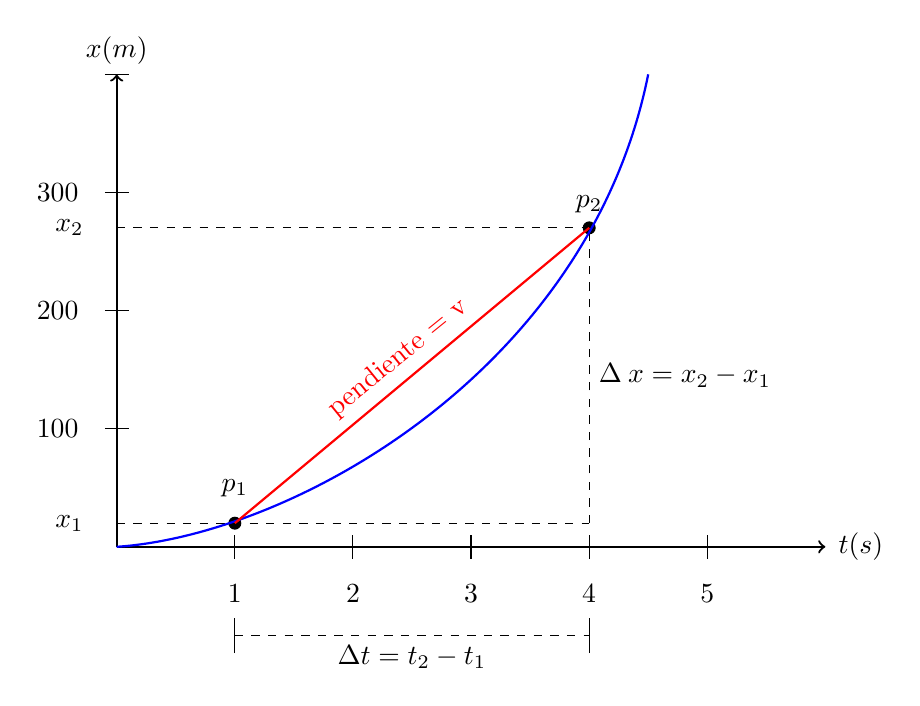
\begin{tikzpicture}[scale=1.5]
% \begin{axis}[
% 		xmin=0, xmax=4,
% 		ymin=0, ymax=400,
% 		xtick={1, 2, 3, 4},     %<--
% 		ytick={100, 200, 300, 400},          %<--
%         xlabel=\($t(s)$\),
%         ylabel=\($x(m)$\)
%         ]
% \end{axis}
	
%    \draw [fill] (1.7, 0.3) circle (0.05);
%    \draw [fill] (6.85, 4) circle (0.05);
    \draw [thick, ->] (0,0) -- (6, 0) node [at end, pos=1.05pt] {$t(s)$};
    \draw [thick, ->] (0,0) -- (0, 4) node [at end, pos=1.05pt] {$x(m)$};
    \foreach \x in {1, 2, 3, 4, 5}{
        \draw (\x, -0.1) -- (\x, 0.1);
        \node at (\x, -0.4) {$\x$};
    }
    \foreach \y in {1, 2, 3, 4}{
        \draw (-0.1, \y) -- (0.1, \y);
    }

    \node at (-0.5, 1) {$100$};
    \node at (-0.5, 2) {$200$};
    \node at (-0.5, 3) {$300$};
    
    \coordinate (p1) at (1, 0.2);
    \coordinate (p2) at (4, 2.7);

    \draw [fill] (p1) circle (0.05);
    \draw [dashed] (0, 0.2) -- (4, 0.2);
    \node at (-0.4, 0.2) {$x_{1}$};
    \node at (1, 0.5) {$p_{1}$};

    \draw [fill] (p2) circle (0.05);
    \draw [dashed] (0, 2.7) -- (4, 2.7);
    \node at (-0.4, 2.7) {$x_{2}$};
    \node at (4, 2.9) {$p_{2}$};

    \draw [dashed] (4, 0.2) -- (4, 2.7) node [midway, right] {$\Delta \: x = x_{2} - x_{1}$};

    %\draw [fill] (1.5, 0.1) circle (0.05);
    %\draw [fill] (4, 1.5) circle (0.05);
    \draw [thick, color=blue] (0, 0) .. controls (1.5, 0.1) and (4, 1.5) .. (4.5, 4);

    \draw (1, -0.9) -- (1, -0.6);
    \draw (4, -0.9) -- (4, -0.6);
    \draw [dashed] (1, -0.75) -- (4, -0.75) node [below, midway] {$\Delta t = t_{2} - t_{1}$};

    %\pause
    \draw [thick, color=red] (p1) -- (p2) node [above, midway, rotate=39] {pendiente = v};
    
\end{tikzpicture}
\end{document}